%!TEX root = ../my_thesis.tex
\subsection{Systematics related to the background subtraction}
\label{sec:syst_mass}
Systematic uncertainties can arise from the choice of the mass fit strategy adopted to calculate \emph{sWeights} (Sec.~\ref{sec:massfit}).
Fit B, used to compute the \emph{sWeights}, is repeated in the full mass window ($[5090,6000]\mevcc$) instead of the narrow signal region ($[5220,5600]\mevcc$).
In this way, the resulting sample is enriched in background events.
The aim of this test is to estimate how much background events (with negative \emph{sWeights}) affect the result for $S_f$ and $S_{\bar f}$ in the final decay time fit.
The fitted total background yield in this new mass fit configuration is $199\,767\pm481$, compared to $34\,102\pm299$ in the nominal fit configuration (Table~\ref{tab:FitBfloating}).
The projection of the PDF used for Fit B in the wide mass range is shown in Fig.~\ref{fig:FitBWideMass}. The new \emph{sWeights} 
are then used in a decay time fit performed on the full sample following the same strategy as reported in Sec.~\ref{sec:datafit}. The correlated disagreement, defined as the difference between the fit results divided by the difference in quadrature between the fitted uncertainties, between the result of this fit and that of the nominal fit is $2.3~\sigma$ for $S_f$ and 
and $1.8~\sigma$ for $S_{\bar f}$. 
Because of this discrepancy, the difference between the newly obtained $S_f$ and $S_{\bar f}$ coefficients and the nominal values is taken as systematic uncertainty, yielding $0.0042$ and $0.0023$ for $S_f$ and $S_{\bar f}$ respectively. The correlation between the systematic uncertainties on $S_f$ and $S_{\bar f}$ is estimated to be $0.7$, as shown in Appendix~\ref{app:corrSyst}.

\begin{figure}[t]
        \begin{center}
                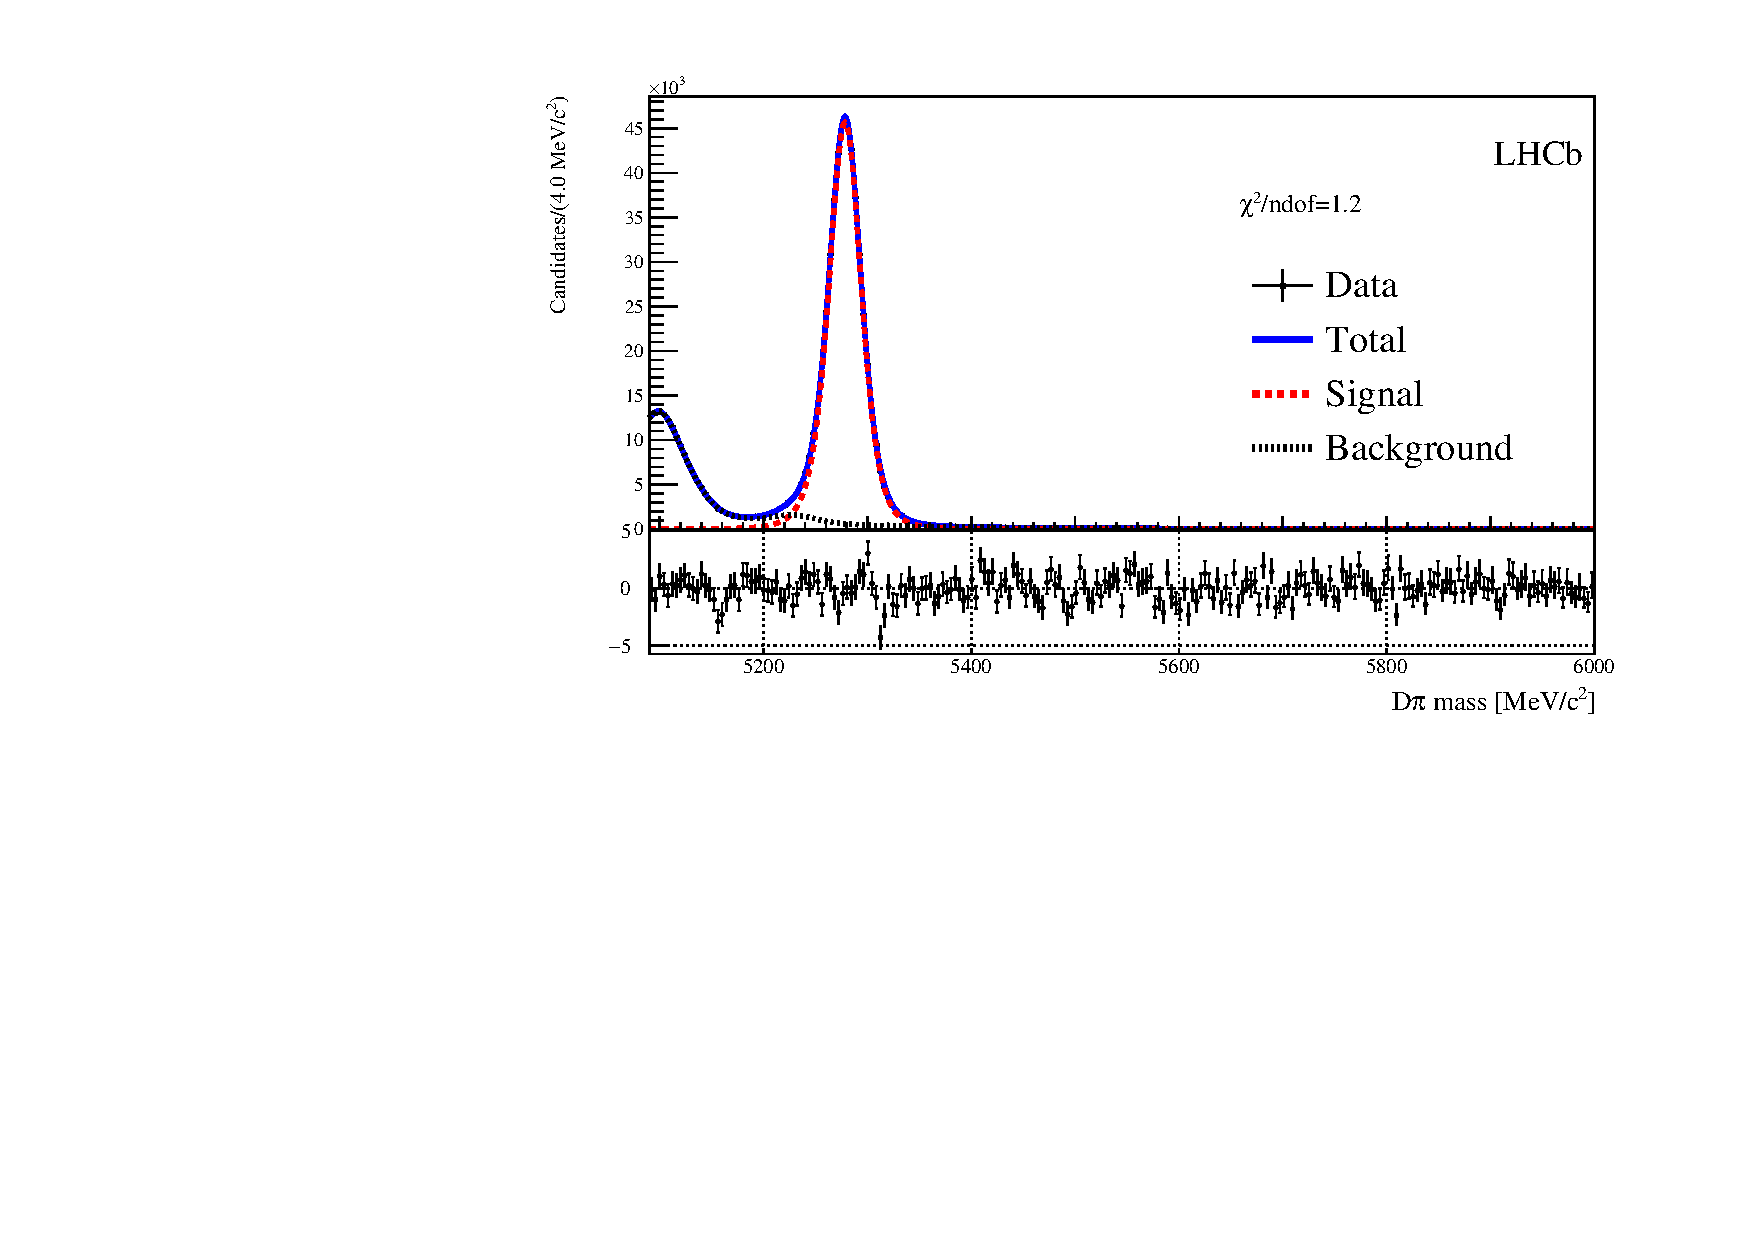
\includegraphics[width=0.7\linewidth]{06Systematics/figs/MDFitPlots_Bd_largeWindow/MDFitForSWeights_BeautyMass_Bd2DPi.pdf}
        \end{center}
        \vspace{-2mm}
        \caption{$\Dmp\pipm$ mass distribution of the $\pi$ sample with the results of Fit B in the large mass window superimposed.}
        \label{fig:FitBWideMass}
\end{figure}

Another test is made by repeating the mass fit with a different strategy:
\begin{itemize}[noitemsep,topsep=0pt]
  \item a $\PIDK<0$ cut (instead of $\PIDK<5$) is applied on the pion PID in order to define the pion sample;
  \item both Fit A and Fit B are performed in the narrow signal region ($[5220,5600]\mevcc$);
  \item during Fit A, only the pion sample is considered (no simultaneous fit in kaon and pion samples is performed);
  \item only $\Bz\to\Dmp\Kpm$ and combinatorial background are considered, whereas all the other physical background are neglected;
  \item the $\Bz\to\Dmp\Kpm$ yield is Gaussian constrained to be $0.0101\pm0.0012$ of the signal yield, based on the selection efficiencies 
    (including the $\PIDK<0$ cut) found on Monte Carlo.
\end{itemize}
The signal and total background yield obtained in this fit are $406\,818\pm674$ and $23\,938\pm266$ respectively.
The projection of the PDF used for Fit A and Fit B in this configuration is shown in Fig.~\ref{fig:MassFitPIDK0}. 
A decay time fit is performed on the resulting sample with \emph{sWeights}
by following the same strategy as reported in Sec.~\ref{sec:datafit}. The correlated discrepancy between the result of this fit and that of the nominal fit is $0.4~\sigma$
and $1.6~\sigma$ for $S_f$ and $S_{\bar f}$ respectively. Given the good level of agreement, and the fact that systematic uncertainties on the PID efficiencies are already considered, no further systematics are assigned.

\begin{figure}[htbp]
        \begin{center}
                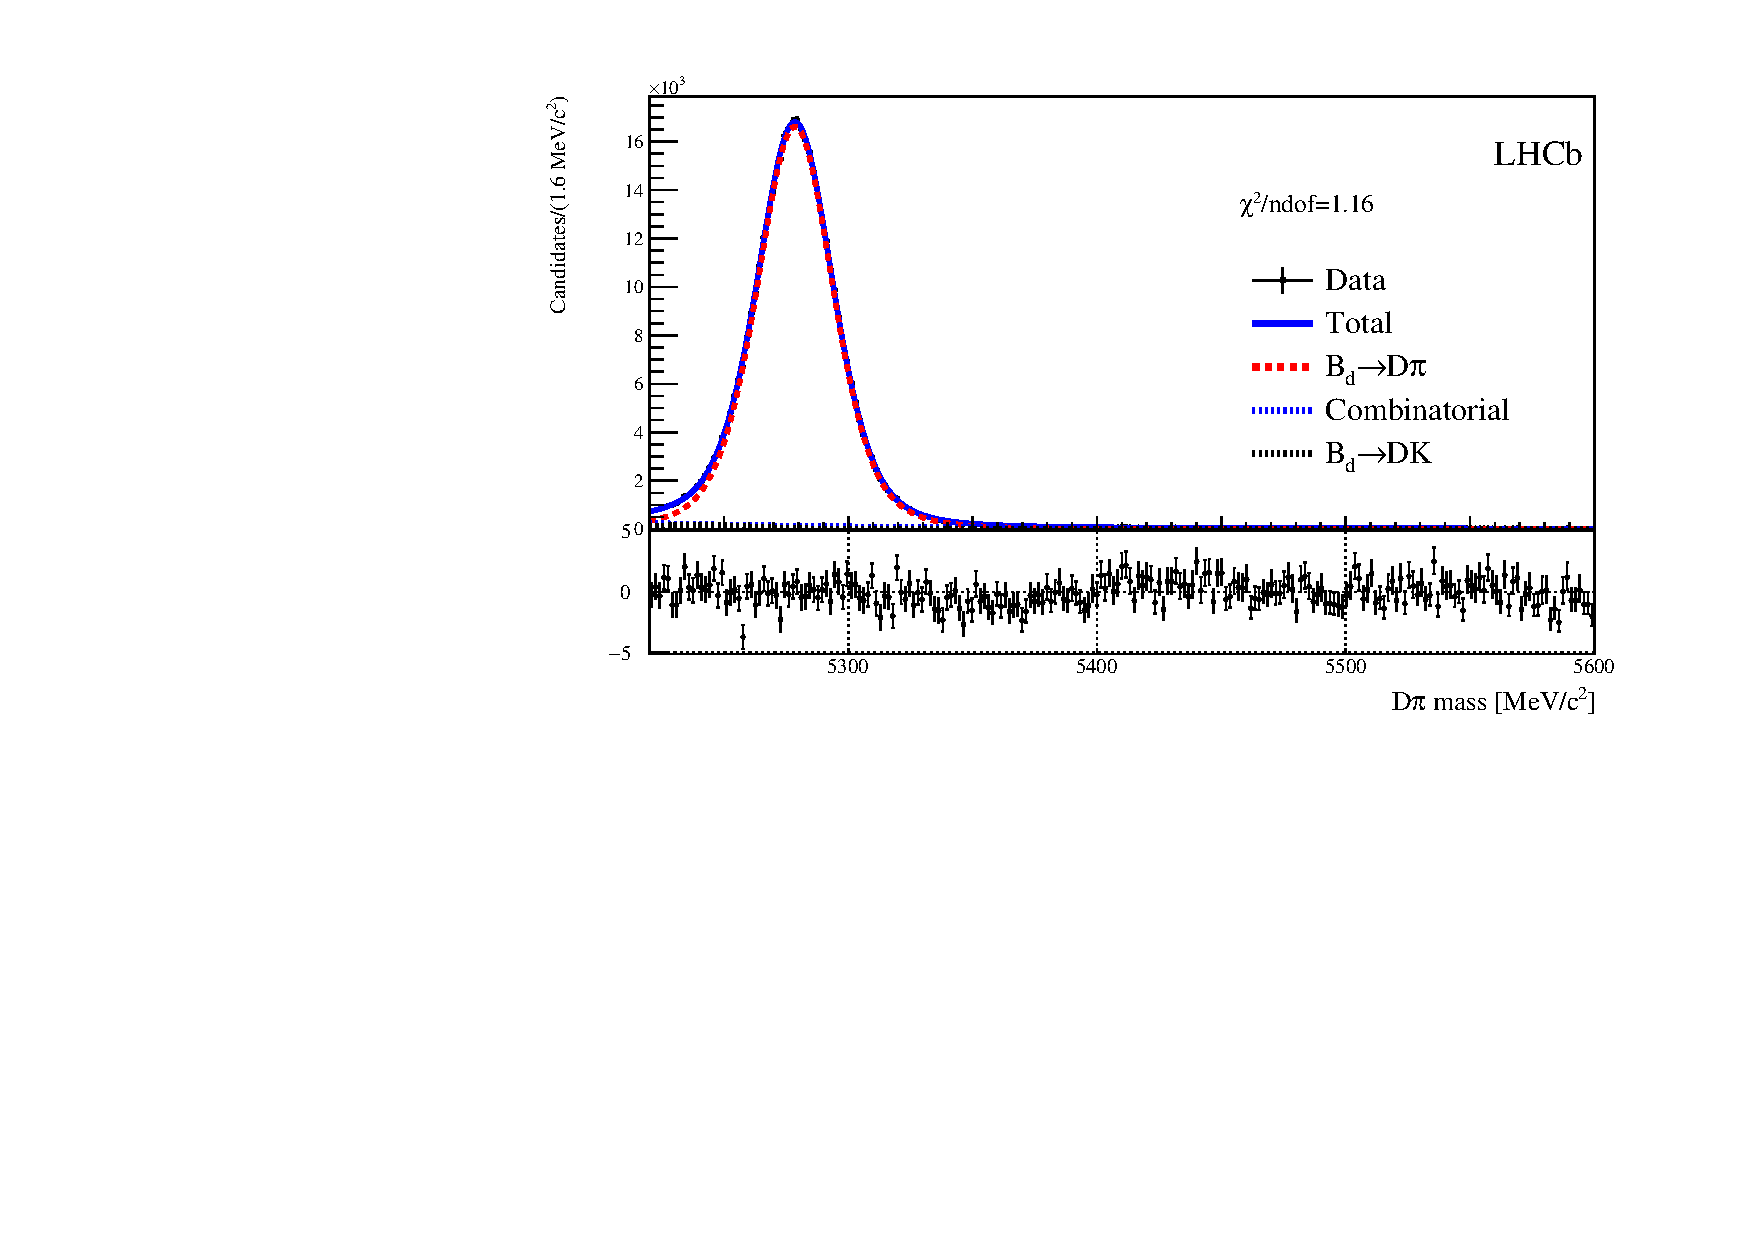
\includegraphics[width=0.49\linewidth]{06Systematics/figs/MDFitPlots_Bd_pidk0/MDFit_BeautyMass_Bd2DPi_withPulls.pdf}
                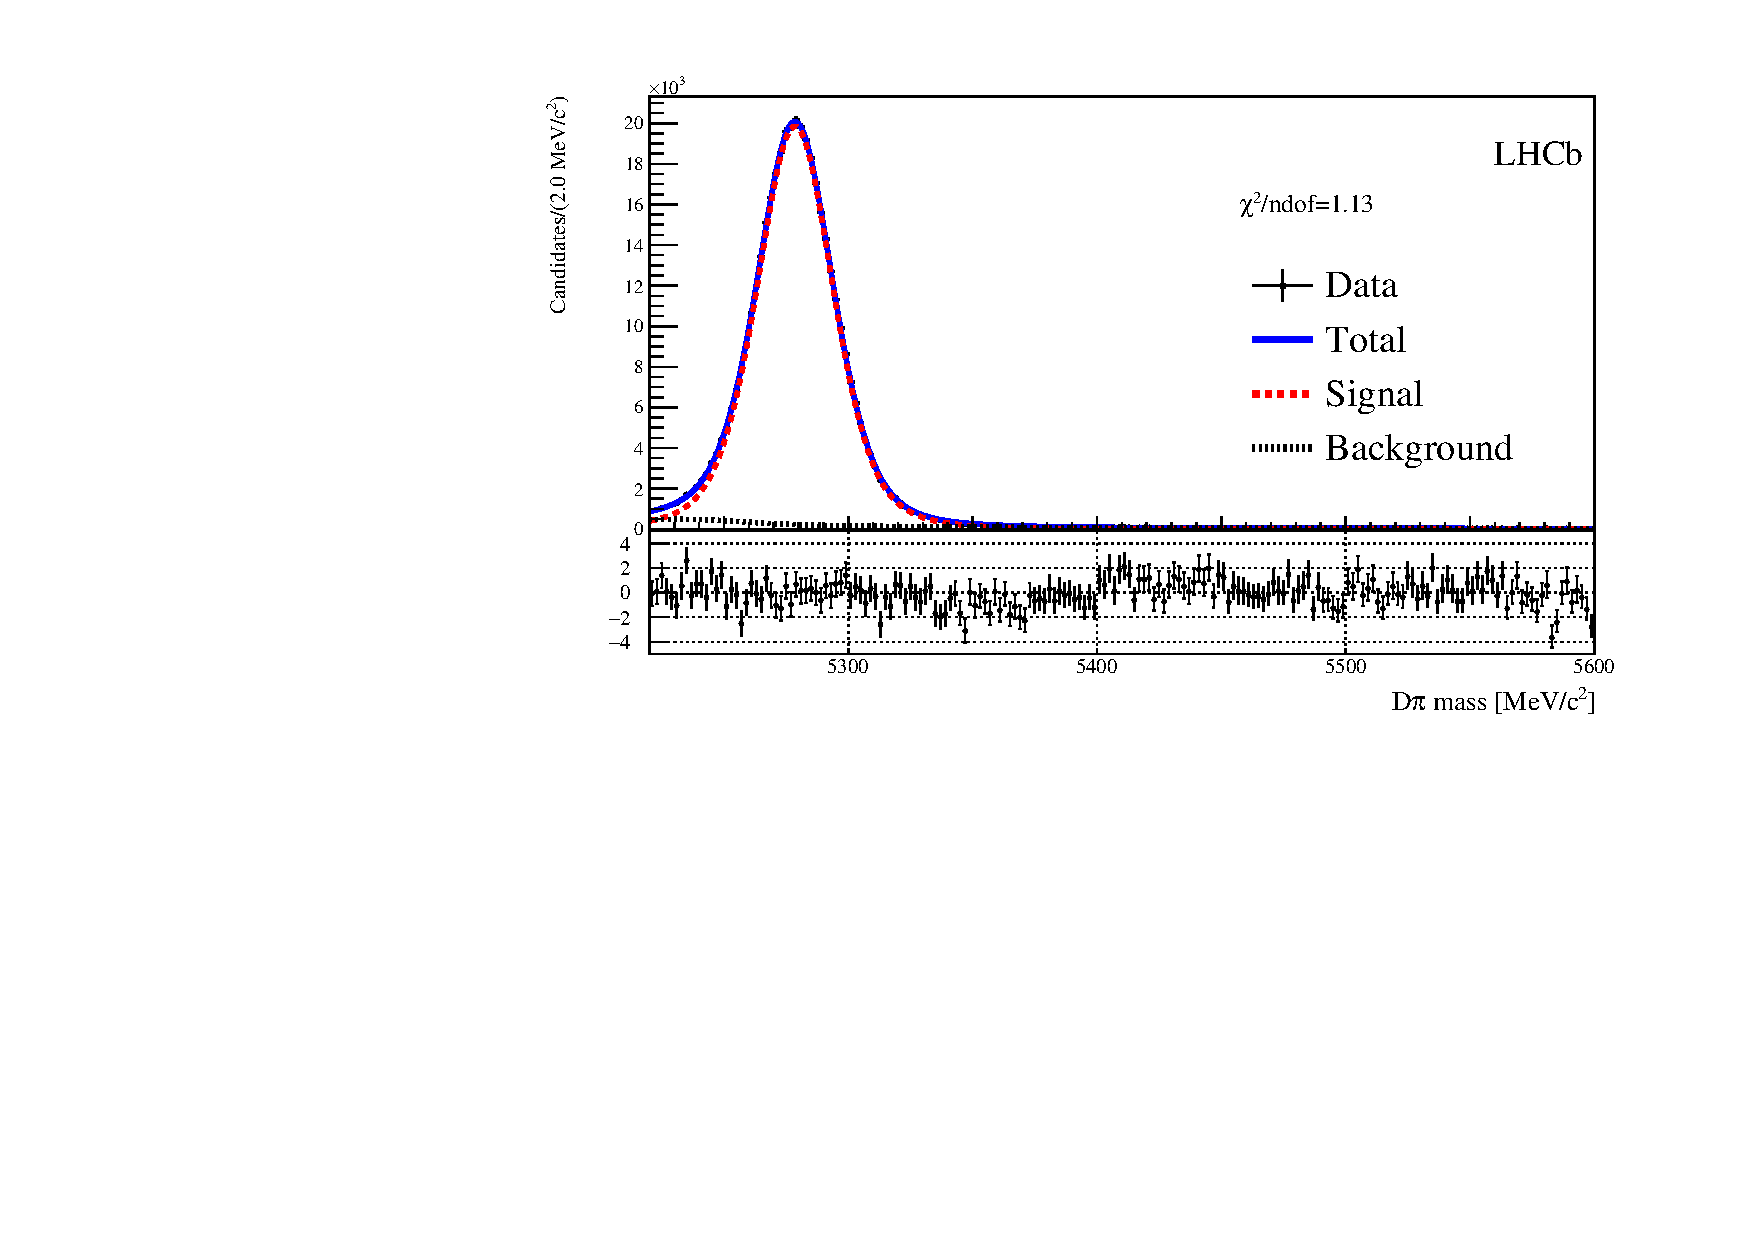
\includegraphics[width=0.49\linewidth]{06Systematics/figs/MDFitPlots_Bd_pidk0/MDFitForSWeights_BeautyMass_Bd2DPi.pdf}
                \end{center}
        \vspace{-2mm}
        \caption{$\Dmp\pipm$ mass distribution of the alternative $\pi$ sample defined by the cut PID$K<0$ on the bachelor pion with the result of Fit A (left) and Fit B (right) superimposed.}
        \label{fig:MassFitPIDK0}
\end{figure}

As additional cross-check, the decay time fit is repeated for $\Bz\to\Dmp\pipm$ candidates restricted in the $[5250,5330]\mevcc$ invariant mass region, very close to
the $\Bz\to\Dmp\pipm$ signal peak position. No \emph{sWeights} are applied on this subsample. 
The correlated disagreement between the result of this fit and that of the nominal fit is $0.2~\sigma$ and $1.3~\sigma$ for $S_f$ and $S_{\bar f}$ respectively. 
Given the good level of agreement, no further systematics are assigned, and the following conclusions are drawn:
\begin{itemize}[noitemsep,topsep=0pt]
  \item the amount of combinatorial and $\Bz\to\Dmp\Kpm$ backgrounds in the signal region is very small,
    and their presence doesn't affect significantly the fitted $S_f$ and $S_{\bar f}$ coefficients as these are compatible with the nominal fit result;
  \item any systematics due to a wrong modelling of signal and/or background PDF in the $\Bz\to\Dmp\pipm$ signal peak region is negligible, since the fitted value obtained from the nominal fit (with \emph{sWeights})
    and this alternative fit (with no mass fit at all) are compatible.
\end{itemize}
